\section{Introduction} \label{sec:introduction}

Robotic packing methods accommodate irregular objects while considering packing density, stability, and placement feasibility~\cite{wang2022binpacking,huang2023binpacking}.
Constructing freestanding structures from natural stones requires finding mutually supporting arrangements among uneven surfaces while achieving a prescribed target shape without support from container walls.

Several stone-stacking methods use placement criteria developed for particular construction settings, including tower-building objectives~\cite{furrer2017stacking} and masonry-inspired geometric rules~\cite{johns2020autonomous,liu2021drystacking}.
For example, Johns et al. generate candidates where target wall surfaces meet the existing structure and apply inward-slope heuristics~\cite{johns2020autonomous}.
Extensions to freeform walls~\cite{johns2023framework} broaden wall geometry; more general targets motivate objectives that use target geometry without wall-specific placement rules.
Structural stability also requires reasoning beyond the support of the newly placed object: its load can affect the equilibrium of objects beneath it.
Liu and Napp~\cite{liu2023stability} explicitly address structural strength during planning, demonstrating the value of evaluating the structure as a whole.
However, assessing the current structure alone does not determine how a placement affects future support and space utilization.
Menezes et al.~\cite{menezes2021rocks} address sequential placement through learned action values that account for future rewards, with a prescribed object sequence and fixed orientations.
We investigate explicit lookahead over object choices and placement poses, coupled with structural stability evaluation and target-shape objectives.

We consider stacking a finite inventory of $n$ irregular objects to approximate a target shape $\target\subset\real^3$.
Let $\object_i(q_i)\subset\real^3$ denote the volume occupied by object $i$ at pose $q_i\in\SE(3)$.
The final configuration objective is
\begin{gather}
\min_{q_1,\cdots,q_n\in\SE(3)} \vol\left(\target\backslash\bigcup_{i=1}^{n}\object_i(q_i)\right)\quad\text{s.t.} \label{eq:problem_definition}\\
c_\text{phys}(\object_1(q_1),\cdots,\object_n(q_n))=0, \nonumber
\end{gather}
where $\vol(\cdot)$ denotes volume and $c_\text{phys}=0$ represents stability and non-interpenetration constraints.
Jointly optimizing all object poses under coupled physical constraints is computationally demanding.
We therefore select one object and optimize its placement at each step, checking the resulting structure's physical feasibility.
Each placement changes support geometry, free space, and remaining inventory, motivating lookahead beyond immediate placement quality.
Our central question is how to combine this lookahead with structural stability evaluation in a common framework for different target shapes.

\begin{figure}[t]
  \centering
  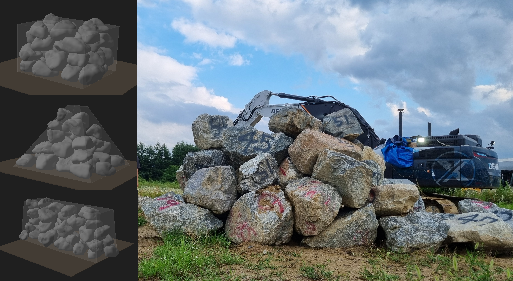
\includegraphics[width=\columnwidth]{figures/preliminary_result.pdf}
  \caption{Preliminary stacking results. Left: simulated structures for different target shapes. Right: a physical stone structure from an outdoor experiment.}
  \label{fig:preliminary_result}
\end{figure}

% Queue the two-column overview on page 1 so it appears at the top of page 2.
\begin{figure*}[t]
  \centering
  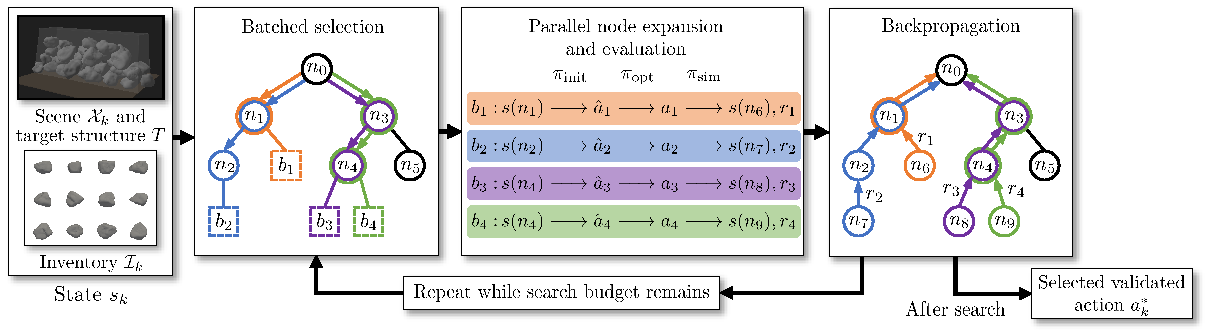
\includegraphics[width=0.94\textwidth]{figures/overview.pdf}
  \caption{Batched MCTS sequence planning. Colors identify expansion requests $b_j$ and their tree paths. Requests are evaluated in parallel through $\initpose$, $\poseopt$, and $\simul$, and returns are backpropagated along the selected paths. Search repeats within the budget before selecting a physically feasible root action $\action_k^*$ from the evaluated tree.}
  \label{fig:overview}
\end{figure*}


Our framework couples bilevel pose optimization with batched, receding-horizon Monte Carlo Tree Search (MCTS)~\cite{huang2022pmbs}.
The optimizer combines target geometry with structure-wide force and torque equilibrium under friction constraints, using bodywise ADMM to parallelize contact-force optimization.
Different targets share this formulation through their geometric representations.
MCTS compares placement sequences using simulation to reject unstable placements and supply settled successor states.

We hypothesize that combining structural stability evaluation with multi-step lookahead improves target coverage while maintaining stability across different target geometries under a fixed planning budget.
Comparisons with greedy placement and candidate-only stability evaluation will test the effects of lookahead and structural coupling, respectively.
Evaluations across target shapes and search horizons will examine the applicability of the common formulation and its computational tradeoffs.
The proposed contributions are:
\begin{itemize}
  \item A bilevel placement optimizer that combines explicit target geometry with contact-force optimization across the structure, using bodywise ADMM updates for GPU computation.
  \item A batched, receding-horizon stacking planner that integrates pose refinement and physical simulation with multi-step lookahead over object choices and placement poses.
\end{itemize}

